\documentclass[extra, camera,%
    onecolumn,   % comment for two columns
    referee,     % uncomment for double lines
    % final,       % uncomment for changes
]{gji}
\usepackage{timet}

% Additional packages
% \usepackage[UKenglish]{babel}
\usepackage[utf8]{inputenc}
\usepackage{lmodern}
\usepackage[T1]{fontenc}
\usepackage{amssymb, amsmath, amsfonts}
\usepackage{booktabs}
\usepackage{xspace}
\usepackage[final]{graphicx}
\usepackage[position=top]{subfig}
\usepackage{ifthen}
\usepackage[addedmarkup=bf]{changes}
% \usepackage[final]{changes}
\usepackage[pdftex, final, allcolors=blue, colorlinks=true]{hyperref}


% workaround siunitx clashes unfortunately with gji
% https://tex.stackexchange.com/a/412886
\makeatletter
\let\zz@tabular\@tabular
\let\zzendtabular\endtabular
\let\zz@xtabularcr\@xtabularcr
\let\zz@tabclassz\@tabclassz
\let\zz@tabclassiv \@tabclassiv 
\let\zz@tabarray\@tabarray
\makeatother

% Figures
% To print widths put this in text:
% \the\textwidth
% \the\columnwidth
%
% Widths:   textwidth  columnwidth  tablewidth
%       1-c   504pt        252pt       504pt
%       2-c   504pt        240pt       240pt
%       ref   468pt        234pt       468pt
%
\newlength{\fwidth}
\newlength{\cwidth}
\newlength{\twidth}
\ifthenelse{\boolean{GJ@referee}}{%
  \setlength{\cwidth}{234pt}%
  \setlength{\fwidth}{468pt}%
  \setlength{\twidth}{468pt}}{%
  \setlength{\fwidth}{504pt}%
  \ifthenelse{\boolean{@twocolumn}}{%
    \setlength{\cwidth}{240pt}%
    \setlength{\twidth}{240pt}}{%
    \setlength{\cwidth}{252pt}%
    \setlength{\twidth}{504pt}%
  }
}
\graphicspath{{./figures/}}

% Change default colour of «changes» package
\definecolor{alizarin}{rgb}{0.82, 0.1, 0.26}
\definecolor{mygreen}{rgb}{0, .5, 0}
\setaddedmarkup{\color{mygreen}{\uline{#1}}}
\setdeletedmarkup{\color{alizarin}{\uwave{#1}}}

\let\tablenum\relax
\usepackage{siunitx}
\usepackage{tabularx}

% To fix clash of gji with hyperref
% https://tex.stackexchange.com/a/384969
\AtBeginDocument{
  \label{CorrectFirstPageLabel}
  \def\fpage{\pageref{CorrectFirstPageLabel}}
}

% Own commands
\newcommand{\mr}[1]{\mathrm{#1}}
\newcommand{\emg}[2]{\texttt{emg#1#2}\xspace}
\newcommand{\empymod}{\texttt{empymod}\xspace}
\newcommand{\simpeg}{\texttt{SimPEG}\xspace}
\newcommand{\custem}{\texttt{custEM}\xspace}

% Remove once done
% \newcommand{\itodo}[1]{\todo[color=blue!40!white, inline]{\sffamily #1}}
% \newcommand{\mtodo}[1]{\todo[inline]{\sffamily #1}}
% \newcommand{\etodo}[1]{\todo[color=blue!40!white]{#1}}
\newcommand{\dul}[1]{\underline{\underline{#1}}}
\newcommand{\ul}[1]{\underline{#1}}
\newcommand{\rmk}[1]{{\color{red}{#1}}}
\newcommand{\ohmm}{\ensuremath{\Omega\,}\text{m}\xspace}
\newcommand{\rtodo}{{\color{red}\texttt{TODO:}}\xspace}

\title[Transforming expensive EM kernels]{Fast Fourier transformation of
electromagnetic data for computationally expensive kernels}

\author[D. Werthmüller \emph{et al.}]
  {\Large
   Dieter Werthmüller$^1$,     % orcid: 0000-0002-8575-2484
   Wim A. Mulder$^{1,2}$ and   % orcid: 0000-0001-7020-9297
   Evert C. Slob$^1$           % orcid: 0000-0002-4529-1134
   \\
   {\footnotesize
    $^1$ TU Delft, Building 23, Stevinweg 1 / PO-box 5048, 2628 CN Delft (NL).
    E-mail: \href{mailto:Dieter@Werthmuller.org}{Dieter@Werthmuller.org}
   }\\[-.3em]
   {\footnotesize
    $^2$ Shell Global Solutions International BV, Grasweg 31, 1031 HW
    Amsterdam(NL)
   }
  }

\date{Received 202Y MMMM DD; in original form 2020 June 30}
\pagerange{\pageref{firstpage}--\pageref{lastpage}}
\volume{VVV}
\pubyear{202Y}


% Authors with AMS fonts and mssymb.tex can comment out the following
% line to get the correct symbol for Geophysical Journal International.
\let\leqslant=\leq

\newtheorem{theorem}{Theorem}[section]

\begin{document}

\label{firstpage}

% workaround siunitx clashes unfortunately with gji
% https://tex.stackexchange.com/a/412886
{\makeatletter
\let\@tabular\zz@tabular
\let\endtabular\zzendtabular
\let\@xtabularcr\zz@xtabularcr
\let\@tabclassz\zz@tabclassz
\let\@tabclassiv \zz@tabclassiv 
\let\@tabarray\zz@tabarray
\maketitle
}
% \maketitle

\begin{summary}
%
Three-dimensional controlled-source electromagnetic data is often computed
directly in the domain of interest, either in the frequency domain or in the
time domain. Computing it in one domain and transforming it via a Fourier
transform to the other domain is a viable alternative. It requires the
evaluation of many responses in the computational domain if standard Fourier
transforms are used. This can make it prohibitively expensive if the kernel is
time-consuming as is the case in three-dimensional electromagnetic modelling.
The speed of such modelling that is obtained through a transform is defined by
three key points: solver, method and implementation of the Fourier
transformation, and gridding.
%
The faster the solver, the faster modelling will be. It is important that the
solver is robust over a wide range of values (frequencies or times). The method
should require as few kernel evaluations as possible while remaining robust. As
the frequency and time ranges span many orders of magnitude, the required
values are ideally equally spaced on a logarithmic scale. The proposed fast
method uses either the digital linear filter method or the logarithmic fast
Fourier transform together with a careful selection of evaluation points and
interpolation. In frequency-to-time domain tests this methodology requires
typically 15 to 20 frequencies to cover a wide range of offsets.
%
The gridding should be frequency- or time-dependent, which is accomplished by
making it a function of skin depth. Optimising for the least number of required
cells should be combined with optimising for computational speed. Looking
carefully at these points results in much smaller computation times with
speedup factors of ten or more over previous methods. A computation in one
domain followed by transformation can therefore be an alternative to
computation in the other domain domain if the required evaluation points and
the corresponding grids are carefully chosen.
%
\end{summary}

% https://academic.oup.com/DocumentLibrary/GJI/gji%20keyword%20list%20updated2017.pdf
\begin{keywords}
  Controlled source electromagnetics (CSEM); Numerical modelling; Fourier
  analysis.
\end{keywords}

\section{Introduction}  % % % % % % % % % % % % % % % % % % % % % % % % % % % %

The controlled-source electromagnetic (CSEM) method is one of the common
non-seismic tools in exploration geophysics, not only in hydrocarbon
exploration \citep{GEO.10.Constable}, but also in the search for sulfides
\citep{GRL.19.Gehrmann}, water \citep{GEO.05.Pedersen}, geothermal sources
\citep{WGC.15.Girard}, or for geological purposes \citep{NAT.19.Johanson}.
While current sources with a few frequencies are used in the deep marine
environment, transient measurements are more common in the shallow marine
environment and on land \citep[e.g., ][]{GEO.07.Ziolkowski, SEG.07.Andreis,
SEG.07.Avdeeva}. One of the main reasons is the dominance of the airwave in
shallow marine and terrestrial measurements, which can be better separated in
the time domain. CSEM is usually divided into frequency- and time-domain
methods, depending on whether the source signal is a continuous waveform, such
as a sine, or a finite waveform, such as a pseudo-random binary sequence
(PRBS). A numerical comparison of the two methods is given by
\cite{GP.13.Conell}. Acquired CSEM data are subsequently often analysed
(modelled and inverted for) in their respective domain, either the frequency or
time domain. Modellers of layered media usually exploit the horizontal
shift-invariance by computing the responses in the wavenumber-frequency domain
followed by a 2D inverse spatial Fourier transform, also called Hankel
transform, to the space-frequency domain, and a regular inverse Fourier
transform if time-domain data are required \citep[e.g., ][]{GEO.15.Hunziker}.

CSEM codes for 2D and 3D computations, on the other hand, mostly compute their
responses directly in the required domain, either frequency or time. There is a
wealth of 3D electromagnetic codes, with a first boom in the 1990's;
\cite{B.SEG.99.Oristaglio} provide a good review of the state of art at that
time. A second wave occurred during the CSEM boom in the hydrocarbon industry
in the early 21th century, see, e.g., \cite{SG.05.Avdeev} and
\cite{SG.10.Borner} for comprehensive overviews. Recent publications after
these review articles span the width of numerical methods from integral
equation codes \citep{MGS.17.Kruglyakov} and differential equation methods such
as finite differences \citep{GEO.10.Mittet, GEO.11.Zaslavsky, CAG.13.Sommer},
finite elements \citep{GJI.13.Grayver}, and finite volumes
\citep{GEO.14.Jahandari}. Besides the different methods there are also many
different types of discretisation. Commonly used, besides rectilinear Yee grids
\citep{IEEE.66.Yee} as used by our code, are Lebedev grids
\citep{CMMP.64.Lebedev} but also unstructured grids using, for instance,
tetrahedra \citep{CAG.17.Cai}. The computational requirement to model CSEM data
also depends heavily on the technique used to solve the system. There are
direct solvers \citep{GEO.15.Grayver}, indirect solvers
\citep{GJI.15.Jaysaval}, and more recently also hybrid solvers
\citep{GEO.18.Liu}.

Under certain conditions it can be a viable alternative to model time-domain
data with a frequency-domain code, as shown by \cite{GEO.08.Mulder}. They
compared the computational complexity of explicit time-stepping schemes (Du
Fort-Frankel method as used in, e.g., \cite{GEO.04.Commer, GEO.07.Maao});
implicit schemes \citep[e.g., ][]{GEO.04.Haber}, and matrix exponentials and
Lanczos reduction schemes \cite[e.g., ][]{RS.94.Druskin} with the Fourier
transform of frequency-domain solutions. Their conclusion was that the Fourier
transform method can be favourable if the number of required frequencies is
small relative to the number of grid points in each coordinate. The conditions
for fast computation of time-domain data with a frequency-domain code are: a
sufficiently powerful solver, appropriate frequency selection and
interpolation, and an automated gridding, for which they used the
multi-frequency CSEM approach presented by \cite{GEO.07.Plessix}. We build upon
these results but improve the run time from hours to minutes. The main reasons
for this significant speed-up are an adaptive, frequency-dependent gridding
scheme that minimizes the required cells in each dimension, and a logarithmic
Fourier transform such as digital linear filters \citep[DLF, ][]{GP.71.Ghosh}
or the logarithmic fast Fourier transform \citep[FFTLog, ][]{RAS.00.Hamilton}
to go from the frequency to the time domain. The latter makes it also possible
to only use the imaginary part of the frequency-domain response, which has
advantages when it comes to interpolation.

While we use the finite-integration technique \citep{AEU.77.Weiland} in the
frequency domain to demonstrate our method, it is important to note that our
ideas can be used with any solver and is not bound to one or another frequency-
or time-domain solver. The ideas for the frequency selection can be applied to
time selection, and time-dependent, adaptive gridding exists as well
\citep[e.g., ][]{RS.06.Commer}. In the next section, we briefly review the
methodology as introduced by \cite{GEO.07.Plessix} and \cite{GEO.08.Mulder} and
highlight their advantages and shortcomings. This is followed by an outline of
our changes to the Fourier transform and the adaptive gridding. Finally, we
demonstrate the efficiency of the approach with some numerical results.

\rtodo \added{Add citation to R.R. (2021) regarding RA and speed-up; limitation
to switch-on/-off.}

\rtodo \added{Add notion about preference for f-domain for IP problems}

\rtodo \added{Extra example: No-IP vs IP; land, 1D}

\section{Motivation}  % % % % % % % % % % % % % % % % % % % % % % % % % % % % %

Being able to model CSEM data both in the frequency domain and in the time
domain can be desirable, as both domains have advantages and disadvantages. One
way to achieve this is to implement Maxwell's equations in both domains.
Another approach is to have Maxwell's equations only implemented in one domain,
and use Fourier transforms to go to the other. However, this approach can be
costly, as many frequencies over a wide range are required to go from the
frequency domain to the time domain, or many times over a wide range for the
opposite direction. We present a methodology which significantly reduces the
amount and range of the required frequencies \added{or times}, translating into
a significant reduction in computation time. The required computation grids for
low frequencies (in our case in the order of 0.001\,Hz) and high frequencies
(around 100\,Hz) are hugely different. Low frequencies can be computed on a
coarser grid, but they require a much larger domain in order to avoid boundary
effects. High frequencies, on the other hand, require denser gridding, but they
are much more limited in reach. An adaptive gridding scheme is therefore
required\replaced{, which}{. We build our approach upon
\mbox{\cite{GEO.07.Plessix}}, who presented such an adaptive gridding for
multi-frequency (and multi-source) CSEM modelling.

An adaptive grid in the frequency domain} is naturally based on the skin depth,
\deleted{which is} the distance after which the amplitude of the
electromagnetic field is decayed by $1/e\approx 37\,\%$. The skin depth
$\delta$ is a function of conductivity and frequency, and for the diffusive
approximation of Maxwell's equations in an isotropic, homogeneous medium is
given by \citep[e.g.,][ equation~1.53]{B.SEG.88.Ward}
%
\begin{equation}
  \delta = \sqrt{\frac{2}{\omega\mu\sigma}}
  \ \approx \ 503.3/\sqrt{f\sigma} \, ,
  \label{eq:skindepth}
\end{equation}
%
where $\sigma$ is conductivity (S/m), $\omega=2\pi f$ is angular frequency of
frequency $f$ (Hz), and $\mu$ is magnetic permeability (H/m). The approximation
is obtained by using the free-space value of magnetic permeability,
$\mu_0=4\pi\times10^{-7}\,$H/m.

\added{We build our approach upon} \cite{GEO.07.Plessix}\added{, who presented
such an adaptive gridding for multi-frequency (and multi-source) CSEM
modelling. They} define the minimum cell width $\Delta_\mathrm{min}$ as
a fraction of the minimum skin depth $\delta_\mathrm{min}$, where
$\delta_\mathrm{min}$ should be 2--3 times bigger than $\Delta_\mathrm{min}$.
The cells have to be smallest around the source; in the marine case, the
minimum skin depth is therefore defined by the conductivity of seawater.
However, this yields quite large cells for low frequencies, so special care has
to be taken around the source by defining a maximum allowed
$\Delta_\mathrm{min}$. The grid dimension, on the other hand, is defined as a
function of the skin depth for the average conductivity of the background,
$\delta_\mathrm{ave}$. They use four times $\delta_\mathrm{ave}$ for the $x$-,
$y$-, and downward $z$-directions, and a fixed 50\,km for the upward
$z$-direction to account for the airwave. To reduce the number of cells, it is
desirable to introduce stretching, at least in the buffer zone outside of the
area where source and receivers are located.

\cite{GEO.08.Mulder} provide a computational complexity analysis of various
methods to model transient electromagnetic responses directly in the time
domain, and compare it to the computation of transient EM responses in the
frequency domain with a subsequent Fourier transform. They conclude the review
by stating \emph{\guillemotleft Although it remains to be seen which of the
four methods requires the least computer time for a given accuracy, the
frequency-domain approach appears to be attractive.\guillemotright} Their
approach is to minimize the computation time by having, in addition to the just
introduced adaptive gridding, an adaptive frequency selection scheme. This
scheme starts with computing the responses for a set of just five frequencies,
regularly sampled on a log-scale, from minimum to maximum required frequency.
All the other frequencies are interpolated with a shape-preserving
piecewise-cubic Hermite interpolation \citep[PCHIP, ][]{SIAM.80.Fritsch}.
Testing the stability of the obtained response by removing a single
frequency-value at a time their scheme decides if more frequencies in-between
the already computed ones are required. In this way frequencies are only added
if required, hence if certain criteria of response stability are not met. While
this method is good and effective for a single offset, it loses all its
advantages if one tries to compute different offsets within one computation, as
each offset requires a different set of adaptive frequencies. Additionally, it
hampers the parallelization over frequencies.

We present improvements to both the adaptive gridding and the transform from
frequency domain to time domain, which makes time-domain modelling with a
frequency-domain code viable in comparison with time-domain codes. It is
important to note that while we show the transform from frequency to time
domain, the conclusions regarding the Fourier transform can equally well be
applied to the transform from time-domain to frequency-domain data for a code
that solves Maxwell's equations in the time domain. \deleted{A variation of our
method was implemented, for instance, by \custem \mbox{\citep{GEO.19.Rochlitz}}
to obtain frequency-domain data from time-domain computations (Rochlitz,
private communication, 2020).}


\section{Methodology} % % % % % % % % % % % % % % % % % % % % % % % % % % % % %

\added{The requirement for any transform is a robust solver of sufficient
precision.} \replaced{We use f}{F}or the numerical computations \deleted{we
use} the open-source (Apache License 2.0) code\added{s \empymod
\mbox{\citep{GEO.17.Werthmuller}} and} \emg3d
\citep{JOSS.19.Werthmuller}\replaced{.}{,} \added{The former computes
semi-analytical responses of layered models, the latter is} a multigrid solver
based on \cite{GP.06.Mulder}, which can be used as a preconditioner for Krylov
subspace solvers or as a solver on its own. The multigrid approach works fine
for the diffusive approximation of Maxwell's equations, which assumes that
$\omega\varepsilon \ll \sigma$, where $\varepsilon$ is electric permittivity
(F/m). The remaining system to solve in the frequency domain is then given by
the second-order differential equation of the electric field,
%
\begin{equation}
    \mathrm{i}\omega\sigma \mathbf{E} +
    \nabla \times \mu^{-1} \nabla \times \mathbf{E}
    = -\mathrm{i}\omega\mathbf{J}_\mathrm{s} \, ,
  \label{eq:maxwell}
\end{equation}
%
where $\mathbf{E}$ is the electric field (V/m) and $\mathbf{J}_\mathrm{s}$ the
current source (A/m$^2$); time dependence is $\exp(\mathrm{i}\omega t)$. The
standard multigrid approach fails for severe stretching or strong anisotropy,
for which known improvements such as line-relaxation and semicoarsening
\citep{ECCFD.06.Jonsthovel} are implemented, with a non-standard Cholesky
decomposition to speed up the computation \citep{GEO.08.Mulder}. One of the big
advantages of the multigrid method is that it scales linearly (optimal) with
the grid size in both CPU and RAM usage \citep{B.Springer.20.Mulder}. This
makes it feasible to run even big models on standard computers, without the
need for big clusters. All the examples in this article are run on a laptop
with an i7-6600U\,CPU\,@\,2.6\,GHz (x4) and 16\,GB of memory, using Ubuntu
20.04 and Python 3.8. All examples were run using a single thread, but
parallelization over frequencies is straight forward, as the computations are
independent. \deleted{For the semi-analytical computations of layered models we
use the open-source (Apache License 2.0) code \empymod
\mbox{\citep{GEO.17.Werthmuller}}.}

\subsection{Frequency selection}  % % % % % % % % % % % % % % % % % % % % % % %

An important factor in terms of speed and accuracy for time-domain responses
obtained from frequency-domain computations is the selection of the required
frequencies. The fewer frequencies required, the quicker we obtain the
time-domain result. \added{This applies primarily for expensive kernels such
as used in 3D modelling where the computation of the response of a single
frequency takes much longer than the transformation itself.} The same applies
for the reverse operation, the fewer times required, the quicker we obtain
frequency-domain results. Even though we limit our analysis here to
frequency-to-time transformations, most of the arguments are reversible and
applicable to time-to-frequency transformations. We decided to use a regular
spacing of frequencies on a log-scale, rather than an adaptive scheme. This
approach is favourable if a wide range of offsets is needed, as the required
frequencies change with offset and an adaptive frequency selection is therefore
often tailored to a single offset\added{ or a limited range of offset}. Also,
it allows for straightforward parallelization over frequencies, which is not
completely possible with an adaptive scheme.

For the actual transform we use either the digital linear filter (DLF) method
or the logarithmic fast Fourier transform (FFTLog). The DLF method was
introduced to geophysics by \cite{GP.71.Ghosh}, and is arguably the most common
method in EM geophysics for both its simplicity and its speed. It is
implemented for the Hankel and Fourier transforms in most EM modelling codes,
e.g., \cite{GEO.09.Key}. A simple tool to design digital linear filters was
recently presented by \cite{GEO.19.Werthmuller}, together with a comprehensive
overview of the history and development of DLF in geophysics. FFTLog,
introduced by \cite{RAS.00.Hamilton}, is another transform algorithm which
proved to be powerful for the frequency-to-time domain transformation of EM
responses, e.g., \cite{INT.14.Werthmuller}. In our tests they are both about
equal in speed and accuracy. DLF requires a wider range and many more
frequencies than the FFTLog. Both methods share some important characteristics
in comparison with the standard FFT: the required input frequencies are equally
spaced on a logarithmic scale (natural logarithm in the case of the DLF and
decimal logarithm in the case of the FFTLog), and they only require either the
real or the imaginary part of the frequency-domain response. We can take
advantage of that by using only the imaginary part of the frequency-domain
response. The imaginary part goes to zero when the frequency goes either to
zero or to infinity, with the advantage that knowing the endpoints makes it
possible to convert the extrapolation of missing frequencies into an
interpolation.

\rtodo \added{Start this section with the method; fmin, fmax, ndec; below we
interpolate with PCHIP, above we set to zero, in-between we interpolate with
cubic spline.}
\replaced{The actually computed frequencies in our approach are defined by
three key-parameters}{There are three key-parameters that have to be defined}:
\replaced{The m}{M}inimum and maximum frequency ($f_\mr{min}, f_\mr{max}$) and
the number of frequencies per decade ($n_\mr{dec}^f$). \added{This creates a
frequency range which is much smaller than the frequency range required for the
transform.} \replaced{A t}{T}rial-and-error \added{approach} with a 3D code is
very time-intensive. However, a simplified, layered model for the required
survey setup and a fast 1D modeller makes it possible to estimate these
parameters easily. \replaced{An example of this is shown in
Figure~\ref{fig:FFTLog-log}.}{To this end, we created a graphical, interactive
tool using \empymod, as shown in Figure~\ref{fig:FFTLog-log}.}
%
\begin{figure}
  \centering
  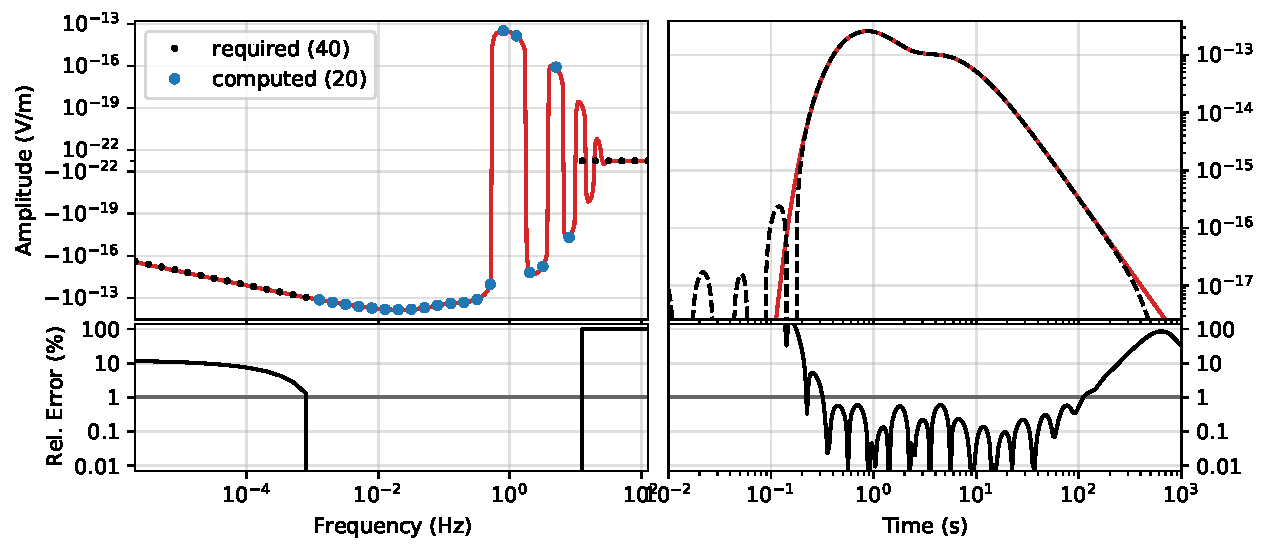
\includegraphics[width=\cwidth]{01-FFTLog-log}
  \caption{\replaced{Example}{Interactive} frequency selection for a
    \replaced{simple}{user-provided} layered model (the shown model parameters
    are described in the text). This example shows the impulse response at an
    offset of 5\,km, for which it uses FFTLog from 0.001\,Hz to 10\,Hz with
    five frequencies per decade. \deleted{Note that the error is clipped for
    values smaller than 0.01\,\% and bigger than 100\,\%.}}
  \label{fig:FFTLog-log}
\end{figure}
%
\replaced{It }{The shown example model} is a marine scenario with 1\,km water
depth of resistivity $\rho=0.3\,\ohmm$ ($\rho = \sigma^{-1}$) and a 100\,m
thick target of 100\,\ohmm at 1\,km below the seafloor in a background of
1\,\ohmm. The source is 50\,m above the seafloor, the receiver is on the
seafloor, and the response is the inline $x$-directed $E$-field. The left
subplot shows the imaginary part in the frequency domain and the right plot the
corresponding impulse response in the time domain. The red lines are the
semi-analytical responses. The blue circles indicate the actually computed
responses and the black dots the frequencies which are interpolated or set to
zero. The resulting time-domain response has a relative error of less than
1\,\% everywhere except for very early times.

Figure \ref{fig:FFTLog-lin} shows exactly the same on a
\replaced{linear}{logarithmic} scale\replaced{for the time and amplitude
axes}{, without the interactive GUI-related elements}. It can be seen that with
the chosen frequencies the time-domain response starts to divert above about
100\,s and below 0.3\,s. It also shows the oscillating high-frequency part,
which is hard to interpolate and we therefore set it to zero.
Figure~\ref{fig:DLF-lin} is the same as Figure \ref{fig:FFTLog-lin}, but
transformed with the DLF method applying the 81-point sine-cosine filter from
\cite{GEO.09.Key}. The same frequencies were computed as in the FFTLog case and
the missing ones interpolated. The error of the corresponding time-domain
response is comparable, so either FFTLog or DLF can be used.
%
\begin{figure*}
  \centering
  \subfloat[]{{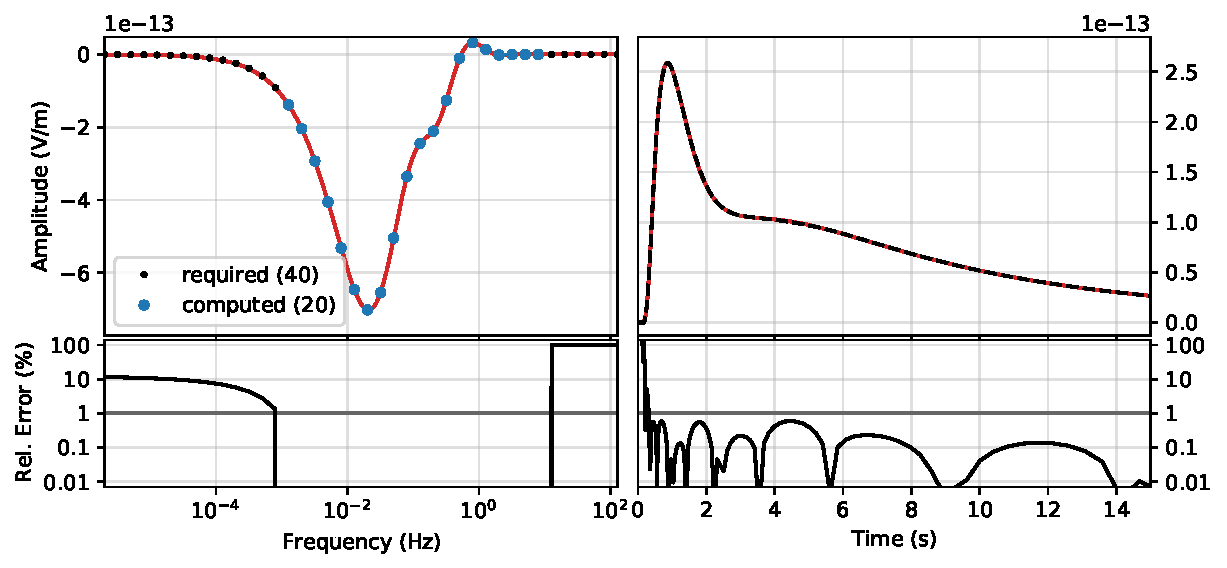
\includegraphics[width=0.5\fwidth]{02a-FFTLog-lin}}%
  \label{fig:FFTLog-lin}}\hfill
  \subfloat[]{{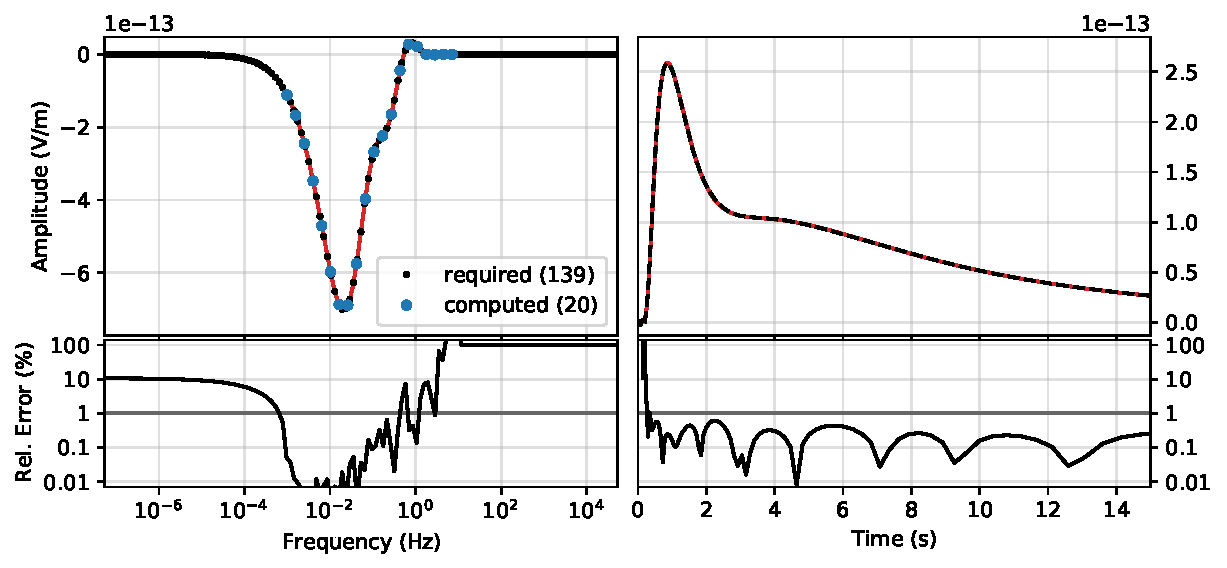
\includegraphics[width=0.5\fwidth]{02b-DLF-lin}}%
  \label{fig:DLF-lin}}\\
  \caption{(a) Same as Figure \ref{fig:FFTLog-log}, but on a logarithmic
  scale. (b) Using DLF instead of FFTLog, but computing the same frequency
  range as for the FFTLog. The resulting time-domain response has comparable
  accuracy\deleted{ (compare the error to the error in Figure
    \ref{fig:FFTLog-log})}.}
  \label{fig:lin-lin}
\end{figure*}
%
In the above example we used 20 frequencies, but that many would not be
required for the shown offset of 5\,km, a few of the lower and higher
frequencies could be left out. With this frequency-selection we can model a
wide range of offsets. This is shown in Figure \ref{fig:multi-offset}, where
the same kernels were used to yield the responses at offsets $r=1.5,3,6$, and
12\,km. We only need to compute 50\,\% of the required frequencies in the case
of the FFTLog, and only 14\,\% in the case of the DLF.
%
\begin{figure*}
  \centering
  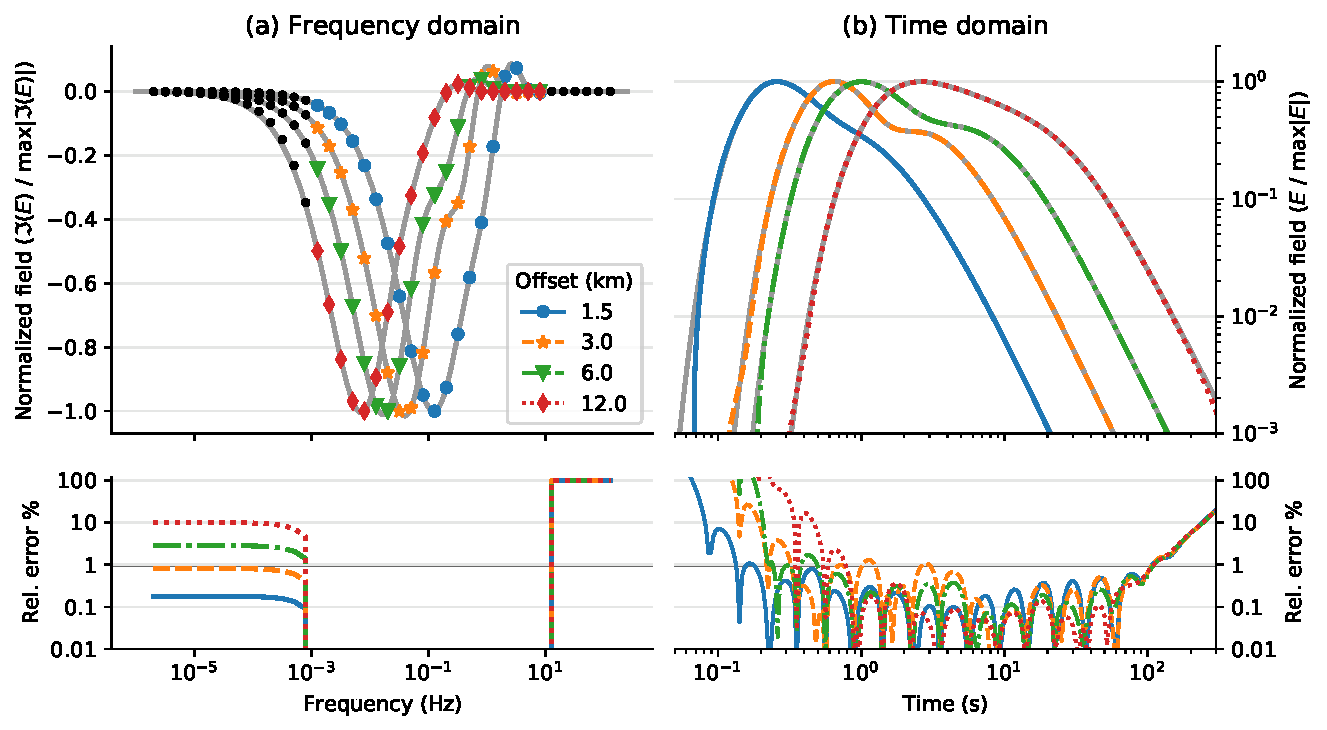
\includegraphics[width=0.75\fwidth]{03-multi-offset}
  \caption{Normalized (a) frequency- and (b) time-domain responses for offsets
    $r=1.5,3,6$, and 12\,km using the parameters defined in Figure
    \ref{fig:FFTLog-lin}. The coloured symbols are the actually computed
    responses, the black dots are the responses which are set to zero (high
    frequencies) or interpolated (low frequencies). The grey curves are the
    analytical responses.}
  \label{fig:multi-offset}
\end{figure*}
%

The shortest offset defines the highest required frequency, and the largest
offset the lowest required frequency. So the more one can restrict the
necessary offset range, the fewer frequencies are needed. Another important
factor is how to interpolate and extrapolate from the computed frequencies to
the frequencies required for the Fourier transform. For the FFTLog only
extrapolation for higher and lower frequencies is required. The EM response
becomes highly oscillatory for high frequencies, which makes it very hard to
extrapolate the response to frequencies $f>f_\mathrm{max}$. However, if
$f_\mathrm{max}$ is chosen judiciously, the importance of higher frequencies
for the Fourier transform can be neglected and we can set those responses to
zero. The extrapolation of frequencies $f<f_\mathrm{min}$ can be changed to an
interpolation by assuming a zero imaginary response at zero frequency, and we
then use PCHIP to interpolate the missing frequencies (as we work on a
logarithmic scale we cannot choose 0\,Hz nor 0\,V/m, but instead take
$10^{-100}$\,Hz and $10^{-100}$\,V/m). In the case of the DLF method we also
have to interpolate in between the computed frequencies, for which we found it
better to use a cubic spline. As can be seen by comparing Figure
\ref{fig:FFTLog-lin} with Figure \ref{fig:DLF-lin}, using the FFTLog or
the DLF with the same actually computed frequencies results in very similar
responses.

The changes to the Fourier transform in comparison with \cite{GEO.08.Mulder}
can be summarized in three points: (1) regular log-scale spacing for the
frequency selection; (2) DLF or FFTLog instead of FFT; and (3) using only the
imaginary part of the frequency-domain response. The actual speed of the
transform is unimportant, as the computation of the frequency-domain responses
takes much longer than the transform itself. What matters is solely how many
frequencies are required by it to achieve the desired precision, and how long
it takes to compute the responses for these frequencies.

\subsection{Gridding}   % % % % % % % % % % % % % % % % % % % % % % % % % % % %

\added{The proposed Fourier transformation requires a robust solver that can
compute precise results over a wide range of frequencies (times) to obtain
time-domain (frequency-domain) responses. In our case the solver uses a
stretched, regular grid and computes the electric fields in the frequency
domain. This setup is the target of the following gridding recommendations.
Whilst they will look differently for other mesh types or a time-domain code,
some conclusion will still hold.}

The computation grid consists of a core or survey domain $D_\mr{s}$ that should
contain all source and receiver positions. The survey domain usually has no or
very little cell stretching factor $\alpha_\mr{s}$. The minimum cell width is
defined as
%
\begin{equation}
  \Delta_\mr{min}=\delta(f, \sigma_\mr{src})/n_\delta \, ,
  \label{eq:minwidth}
\end{equation}
%
where $\sigma_\mr{src}$ is the conductivity of the media in which the source
resides, and $n_\delta$ is a positive number that defines how many cells there
should be per skin depth. The actual computational domain $D_\mr{c}$ is usually
much bigger than $D_\mr{s}$ in order to avoid artefacts from the perfectly
electrically conducting boundary condition. It can also have a much higher
stretching factor $\alpha_\mr{c}$. In the presented examples we have chosen
$D_\mr{c}$ such that the distance for the signal diffusing from the source to
the boundary and back to the receiver closest to the boundary is at least two
wavelengths, after which the amplitude of the signal is reduced to a millionth
of its initial strength. The wavelength $\lambda$ to compute $D_\mr{c}$ is
given by
%
\begin{equation}
  \lambda = 2\pi\delta(f, \sigma_\mr{ave})
  \ \approx \ 3162/\sqrt{f\sigma_\mr{ave}}\, ,
 \label{eq:lambda}
\end{equation}
%
where $\sigma_\mr{ave}$ is the average conductivity, which can vary for
different directions. However, the skin-depth approach fails for air, in which
the EM field propagates as a wave at the speed of light. A largest
computational domain is therefore enforced, defining the maximum distance from
the source to the boundary; this distance is by default set to 100\,km, but
this can be reduced in the marine case with increasing water depth. Note that
for shallow marine and land cases this also applies to the horizontal
dimensions, not only to the upward $z$-direction and similarly for very
resistive basements, even in deep water. One way to circumvent this difficulty
is the use of a primary-secondary formulation, where the primary field,
including the air wave, is computed with a semi-analytical code for layered
media. We do not consider this approach here. \added{Note that grid stretching
for complex-valued diffusion fields is essentially what is done for wave fields
with the perfectly matched layer (PML). PML is an absorbing layer to avoid
scattering from the boundary by letting the field die out to zero, which is
achieved by introducing a complex factor which causes damping. As
electromagnetic diffusion fields are damped fields by themselves it suffices to
stretch the grid.}

In summary, the adaptive gridding takes $f$, $D_\mr{s}$, $\sigma_\mr{src}$,
$\sigma_\mr{ave}$, $n_\delta$, and ranges for $\alpha_\mr{s}$, $\alpha_\mr{c}$,
where we usually fix $\alpha_\mr{s}=1$ or keep it at least below 1.05, and let
$\alpha_\mr{c}$ be anything between $[1, 1.5]$. The minimum cell width
$\Delta_\mr{min}$ can further be restricted by a user-defined range. Given
these inputs, the adaptive gridding will search for the smallest possible
number of cells which fulfils these criteria. The implemented multigrid method
puts some constraints on the number of cells, of which the adaptive gridding
takes care (the number of cells have to be powers of two multiplied by a low
prime, e.g., $\{2,3,5\}\cdot2^n$).

The main difference with \cite{GEO.08.Mulder} is that their adaptive gridding
searches for the optimal stretching factor $\alpha$ fulfilling certain
criteria, for a fixed number of cells. Our adaptive gridding, on the other
hand, searches for the smallest number of cells that still fulfils the given
criteria. The number of cells becomes therefore also a function of frequency.
It is important to note that this is our implementation of an adaptive grid,
but there are certainly other possibilities. The relevant point for fast
computations is that the adaptive gridding tries to minimize the number of
required cells. This is generally best done in a frequency- and
conductivity-dependent manner. To go from the model grid to the computational
grid, we use the volume-averaging technique on logarithmic resistivities, as
used in \cite{GEO.07.Plessix}. While this technique ensures that the total
resistivity in the subsurface remains the same, it does not consider
effective-medium theory \citep{GEO.03.Davydycheva}, for instance, the apparent
anisotropy from a stack of finely layered formations of varying resistivity.


\section{Numerical examples}  % % % % % % % % % % % % % % % % % % % % % % % % %


\subsection{Homogeneous space}  % % % % % % % % % % % % % % % % % % % % % % % %

The first example is the inline electric field from a source at the origin
measured by an inline receiver with an offset of 900\,m in a homogeneous space
of 1\,\ohmm. We chose this simple example to compare it with the analytical
solution and with previously published results. We used the following values to
define the required frequencies: $f_\mr{min}=0.05\,$Hz, $f_\mr{max}=21\,$Hz,
using FFTLog with 5 frequencies per decade. This results in 14 frequencies to
compute from 0.05\,Hz to 20.0\,Hz. The complete frequency range for the
transform, including the frequencies for which we use interpolation, includes
30 frequencies from 0.0002\,Hz to 126.4\,Hz. For the adaptive gridding the
following inputs were used: $n_\delta=12$, minimum cell width must be between
20 and 40\,m, and $\alpha_\mr{s}=1$, $\alpha_\mr{c}=[1,1.3]$. This yields grids
with cell numbers between \num{46080} ($80\times24\times24$, for 20.0\,Hz) and
\num{128000} ($80\times40\times40$, for 0.05\,Hz) cells. The run times for each
frequency, the corresponding number of cells, minimum cell width, and
computation domain stretching factor are listed in Table~\ref{tbl:timefull}.
The total run time to compute this model was less than two minutes.
%
\begin{table}
\begin{minipage}{\twidth}
  \centering
  \caption{Run times per frequency for the homogeneous space example, with the
    corresponding number of cells and minimum cell width as well as the
    stretching factor in the computation domain; $\alpha_\mr{s}=1$ everywhere.}
  \label{tbl:timefull}
  \begin{tabular}{S[table-format=2.4]rrrr}
    \toprule
    %
    {Frequency} & Time & nx$\times$ny$\times$nz & $\Delta_\mr{min}$ & $\alpha_\mr{c}$ \\
    {(Hz)}  & (s) &  & (m) & \\
    \midrule
    %
    20.0    &  4 & 80$\times$24$\times$24 & 20 & 1.26 \\
    12.6    &  8 & 96$\times$32$\times$32 & 20 & 1.17 \\
     7.98   &  8 & 96$\times$32$\times$32 & 20 & 1.20 \\
     5.03   &  8 & 96$\times$32$\times$32 & 20 & 1.23 \\
     3.18   &  7 & 80$\times$32$\times$32 & 24 & 1.23 \\
     2.00   &  7 & 80$\times$32$\times$32 & 30 & 1.21 \\
     1.26   &  5 & 64$\times$32$\times$32 & 37 & 1.21 \\
     0.798  &  5 & 64$\times$32$\times$32 & 40 & 1.23 \\
     0.503  &  5 & 64$\times$32$\times$32 & 40 & 1.26 \\
     0.318  &  5 & 64$\times$32$\times$32 & 40 & 1.28 \\
     0.200  &  8 & 64$\times$40$\times$40 & 40 & 1.27 \\
     0.126  &  8 & 64$\times$40$\times$40 & 40 & 1.30 \\
     0.0798 & 10 & 80$\times$40$\times$40 & 40 & 1.26 \\
     0.0503 & 11 & 80$\times$40$\times$40 & 40 & 1.28 \\
    %
    \bottomrule
  \end{tabular}
\end{minipage}
\end{table}
%

Figure \ref{fig:fullspace} (a) shows the frequency-domain result, where the
blue dots are the computed responses and the black dots correspond to the
interpolated values or the values set to zero.
%
\begin{figure*}
  \centering
  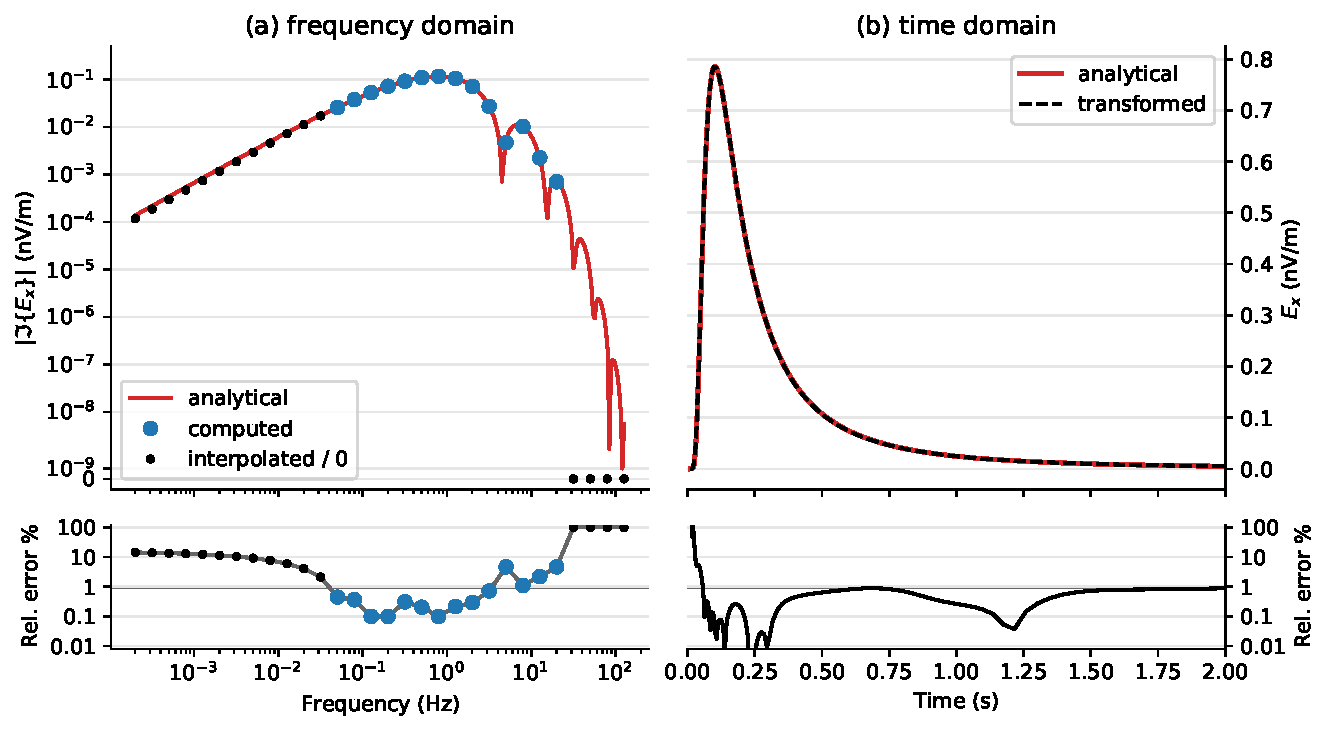
\includegraphics[width=\fwidth]{04-fullspace}
  \caption{(a) Frequency- and (b) time-domain results for the homogeneous space
    model. The red lines are the analytical solutions, the blue circles are the
    actually computed responses, the black dots are the interpolated responses,
    and the dashed black line the obtained time-domain response. \deleted{The
    errors are clipped for values smaller than 0.1\,\% and bigger than
    100\,\%.}}
  \label{fig:fullspace}
\end{figure*}
%
Most of the computed values stay below a relative error of 1\,\%, our chosen
adaptive gridding only starts to generate considerable errors at higher
frequencies. Figure \ref{fig:fullspace}(b) shows the corresponding time-domain
result, where the dashed black line is the result obtained by transformation of
the frequency-domain response, on top of the red line which is the analytical
result. The relative error is mostly below 1\,\%, except for early times.
However, for practical reasons that is more than enough.
Figure~\ref{fig:fullspace-log} shows the same on a logarithmic scale, with
times up to 10 seconds. It clearly shows that if later times are required, we
would need to adjust our Fourier transform parameters.
%
\begin{figure}
  \centering
  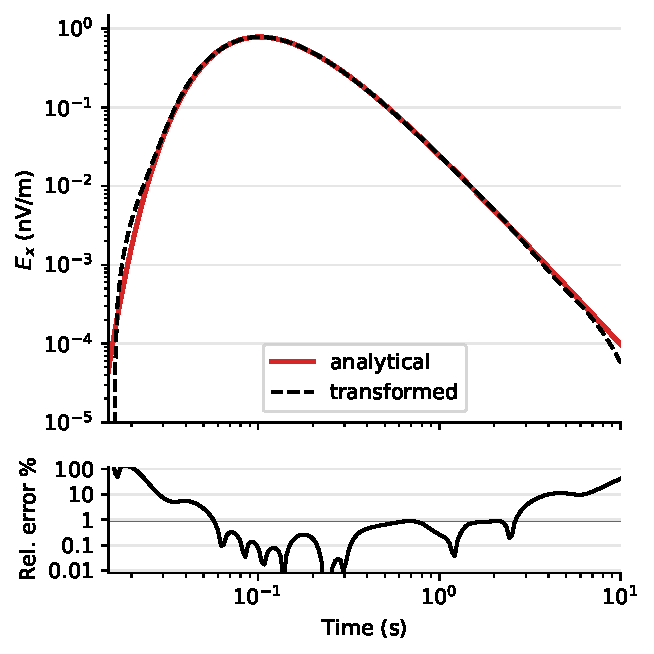
\includegraphics[width=\cwidth]{05-fullspace-log}
  \caption{Same as in Figure~\ref{fig:fullspace} (b), but on a logarithmic
    scale. To improve later times we would have to compute lower frequencies;
    to improve earlier times we would have to compute more frequencies per
    decade to get a better resolution.}
  \label{fig:fullspace-log}
\end{figure}
%
Note that for the gridding we chose $n_\delta=12$, which is very dense. This
was necessary because we are relatively close to the source. If the offsets of
interest are larger this factor can be lowered considerably; 3--4 is often
enough.

This model corresponds to the one presented in Table 1 and in Figures 3 and 4
of \cite{GEO.08.Mulder}. The response here appears to be more accurate, their
reported peak-error is roughly 1\,\%, whereas we are below 0.1\,\% at the peak
(there are no error-plots presented, so visual inspection is all we have).
However, the difference in run time is dramatic. Summing the run times for the
different frequencies of the original figure comes to a total computation time
of 3\,h 47\,min 12\,s; 0.01\,Hz was the slowest run with 31\,min 19\,s, and
2.37\,Hz was the fastest run with 2\,min 54\,s. Our example, on the other hand,
took less than two minutes in total, where the individual frequencies took
between 4 and 11\,s to run.

This massive speed-up has a couple of reasons. Computers have become more
powerful in the last twelve years, and the codes were run on different
computers. A quick test with the old scripts on our test machine shows that it
would roughly run 2--3 times faster, therefore somewhere between 1 and 2 hours.
The more important facts besides different hardware are: (1) we only used 14
frequencies instead of the 26 frequencies between 0.01 and 100\,Hz of the
original; (2) our adaptive gridding used significantly less cells
($f$-dependent) in comparison to the fixed \num{2097152} cells ($128^3$) used
in the original example. We did not see a significant difference in the speed
of the actual codes, where the kernel-algorithm of the two implementations is
the same, but in the original example it is implemented in Matlab/C, whereas
\emg3d is written in Python/Numba (Numba is a just-in-time compiler for Python
code, \cite{Numba}).


\subsection{1D Model} % % % % % % % % % % % % % % % % % % % % % % % % % % % % %

The second example is a shallow marine, layered model with 200\,m of seawater
(3\,S/m) above a halfspace of 1\,S/m, an embedded target layer at 2\,km depth,
100\,m thick, with a conductivity of 0.02\,S/m. The source is located 20\,m
above the seafloor and the receivers are on the seafloor. We chose the
frequency range such that we can model offsets from 3 to 7 kilometers, with
$f_\mr{min}=0.007\,$Hz and $f_\mr{max}=32\,$Hz, using FFTLog with 5 frequencies
per decade. This results in computations for 19 frequencies from 0.008\,Hz to
31.8\,Hz. The complete frequency range for the transform includes 35
frequencies from $2\,10^{-5}$ to $126.4\,$Hz. For the adaptive gridding, we
used a cell width of 100\,m in the core domain and stretching outside up to a
factor 1.5, where the computation domain extends up to 50\,km in each
direction. This yielded grids between \num{204800} (higher frequencies) and
\num{245760} (lower frequencies) cells. The run times for each frequency and
their corresponding parameters are listed in Table~\ref{tbl:timemarine}.
%
\begin{table}
\begin{minipage}{\twidth}
  \centering
  \caption{Run times per frequency for the marine 1D example, with the
    corresponding number of cells and minimum cell width as well as the
    stretching factor in the computation domain; $\alpha_\mr{s}=1$ everywhere.}
  \label{tbl:timemarine}
  \begin{tabular}{S[table-format=2.5]rrrr}
    \toprule
    %
    {Frequency} & time & nx$\times$ny$\times$nz & $\Delta_\mr{min}$ & $\alpha_\mr{c}$ \\
    {(Hz)}  & (s) &  & (m) & \\
    \midrule
    %
    31.8     & 16 & 128$\times$40$\times$40 & 100 & 1.36 \\
    20.0     & 17 & 128$\times$40$\times$40 & 100 & 1.36 \\
    12.6     & 17 & 128$\times$40$\times$40 & 100 & 1.36 \\
     7.98    & 17 & 128$\times$40$\times$40 & 100 & 1.36 \\
     5.03    & 17 & 128$\times$40$\times$40 & 100 & 1.44 \\
     3.18    & 17 & 128$\times$40$\times$40 & 100 & 1.48 \\
     2.00    & 17 & 128$\times$40$\times$40 & 100 & 1.49 \\
     1.26    & 20 & 128$\times$40$\times$48 & 100 & 1.36 \\
     0.798   & 24 & 128$\times$40$\times$48 & 100 & 1.36 \\
     0.503   & 27 & 128$\times$40$\times$48 & 100 & 1.36 \\
     0.318   & 27 & 128$\times$40$\times$48 & 100 & 1.36 \\
     0.200   & 34 & 128$\times$40$\times$48 & 100 & 1.38 \\
     0.126   & 34 & 128$\times$40$\times$48 & 100 & 1.40 \\
     0.0798  & 37 & 128$\times$40$\times$48 & 100 & 1.41 \\
     0.0503  & 37 & 128$\times$40$\times$48 & 100 & 1.44 \\
     0.0318  & 44 & 128$\times$40$\times$48 & 100 & 1.44 \\
     0.0200  & 44 & 128$\times$40$\times$48 & 100 & 1.47 \\
     0.0126  & 37 & 128$\times$40$\times$48 & 100 & 1.48 \\
     0.00798 & 43 & 128$\times$40$\times$48 & 100 & 1.49 \\
    %
    \bottomrule
  \end{tabular}
\end{minipage}
\end{table}
%

Figure~\ref{fig:marine} shows the result for an offset of 5\,km, in (a) the
frequency and (b) the time domain. The recovered response with the 3D code
captures the airwave (first peak) and the subsurface (second peak) very
accurately. At later times the error starts to increase. We would need to
compute a few additional lower frequencies if we want to improve it.
%
\begin{figure*}
  \centering
  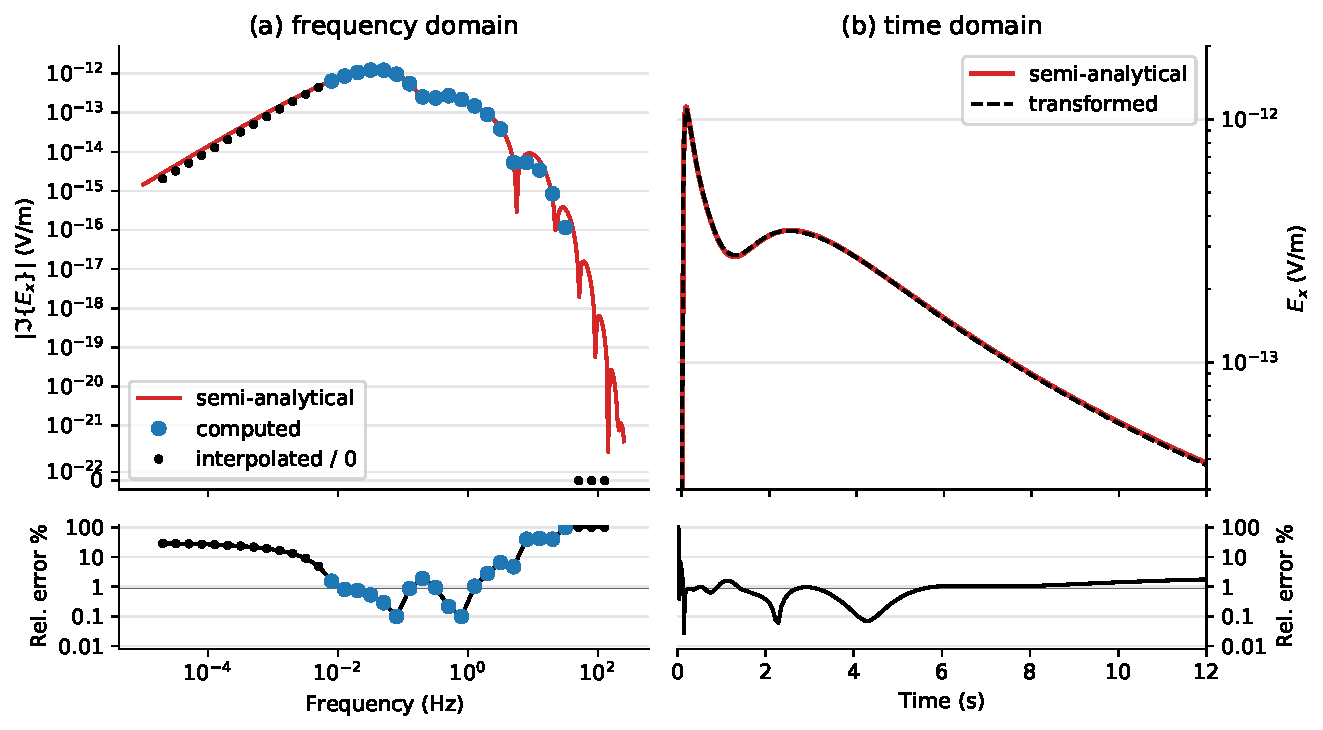
\includegraphics[width=\fwidth]{06-marine}
  \caption{Electric inline response at an offset of 5\,km for a shallow marine,
    layered scenario. (a) Frequency-domain response, where the blue circles
    denote computed responses and the black dots interpolated responses or
    responses set to zero. (b) Time-domain response.}
  \label{fig:marine}
\end{figure*}
%
In the frequency-domain plot, it can be seen that the high frequencies are not
computed very accurately, but without too much influence on the time-domain
response. These frequencies could be left out if an offset of 5\,km is the only
objective. However, we also want to retrieve shorter offsets from the same
computation, for which these frequencies are required.

Figure~\ref{fig:marine-multioffset} shows the time-domain responses of the same
model for offsets of 3, 5, and 7\,km, all obtained with the same
frequency-domain computations and the same frequencies for the Fourier
transform. The computation of these frequencies took less than 9 minutes and it
handles any offset between 3 and 7\,km. It can be seen that the chosen
frequency selection is sufficient for this offset range; again, more low
frequencies could be added to improve late-time values.
%
\begin{figure}
  \centering
  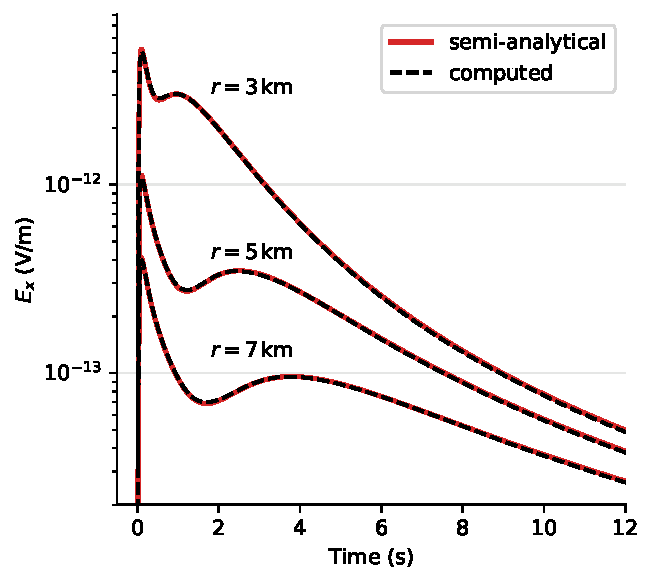
\includegraphics[width=\cwidth]{07-marine-multioffset}
  \caption{Time-domain responses for offsets of 3, 5, and 7\,km for the same
    model as shown in Figure~\ref{fig:marine}.}
  \label{fig:marine-multioffset}
\end{figure}
%


\subsection{Horizontal extent of the computation domain}  % % % % % % % % % % %

The skin-depth approach fails for the air layer, as explained in the Section
\emph{Gridding}. The reason is that the EM field in the air travels at the
speed of light as a wave, and its amplitude is only reduced through geometrical
spreading. On land and in shallow marine scenarios one has therefore to include
a sufficiently large computational domain. The default in our scheme is
100\,km. The important point is that this does not only apply to the upward
$z$-direction, but also to the horizontal directions, as the airwave bounces
back horizontally and would continuously emit energy into the subsurface if the
boundaries are not chosen far enough away from the receivers. If models are
computed with very resistive layers or models with highly resistive basements,
this can even apply to deep marine scenarios.

Figure~\ref{fig:marine-wrong-x-y} shows this effect. It is the same model as in
the previous section; however, for the adaptive gridding in the horizontal
directions, $\rho_\mr{ave}=1\,\ohmm$ was used instead of
$\rho_\mr{ave}=\num{10000}\,\ohmm$. Having the boundaries too near in the
horizontal directions leads to worse results for most frequencies and entirely
wrong results for high frequencies. Comparison with the 1D result in the time
domain shows that it is the airwave whose amplitude is heavily overestimated.
%
\begin{figure*}
  \centering
  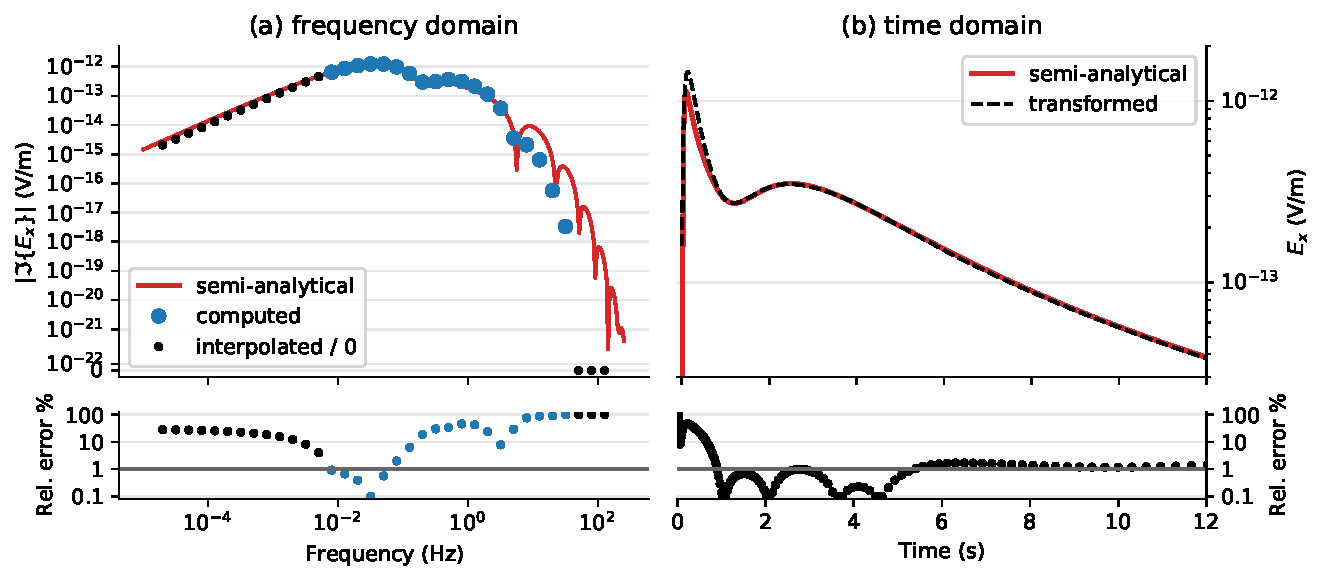
\includegraphics[width=\fwidth]{08-marine-wrong-x-y}
  \caption{Same model as used for Figure~\ref{fig:marine}, but with the
    horizontal boundaries not far enough. Although the resulting time-domain
    result looks plausible, the comparison with the 1D result shows that it
    significantly overestimates the amplitude of the airwave.}
  \label{fig:marine-wrong-x-y}
\end{figure*}
%
It can be difficult to spot these errors in the time-domain result, as the
response looks plausible. Only a comparison with the 1D result reveals that it
is actually wrong. A possibility to detect such problems for complicated cases,
where there is no semi-analytical result to compare with, is to compute two or
more models, moving the boundary. When the responses stop to change, one can
assume that the boundary is far enough. Another possibility is to look at the
amplitudes close to the boundaries and ensure that they are small enough.


\subsection{3D Model} % % % % % % % % % % % % % % % % % % % % % % % % % % % % %

The final example consists of a resistive, three-dimensional block embedded in
the lower of two halfspaces, as depicted in Figure~\ref{fig:3d-model}. The
target has resistivity $\rho_\mr{tg}=100\,\ohmm$, the upper halfspace
corresponds to seawater with $\rho_\mr{sea}=0.3\,\ohmm$, and the lower
halfspace is the background with $\rho_\mr{bg}=1\,\ohmm$.
%
\begin{figure}
  \centering
  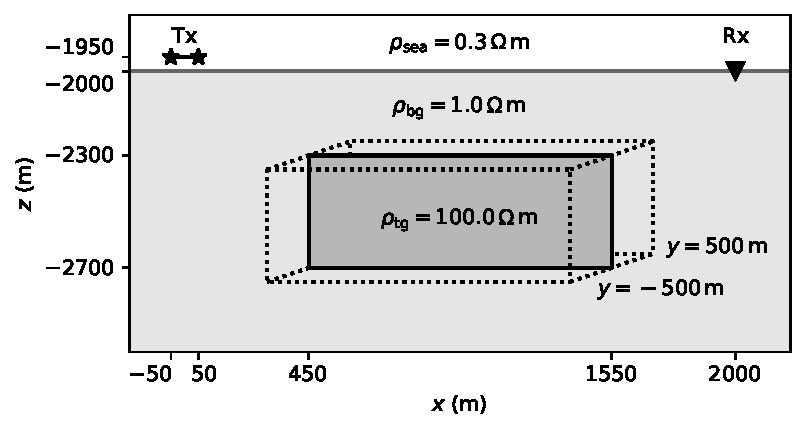
\includegraphics[width=\cwidth]{09-3d-model}
  \caption{Three-dimensional block embedded in the lower of two halfspaces. The
    100-m long, $x$-directed dipole source is located 50\,m above the seafloor
    at the origin, and the receiver is on the seafloor at an offset of 2\,km.}
  \label{fig:3d-model}
\end{figure}
%
The source is a 100-m long, $x$-directed dipole at the origin, 50\,m above the
seafloor, and we are using a step-off source function. The $x$-directed inline
receiver is at an offset of 2\,km. The dimension of the target cube is
$1.1\times1.0\times0.4$\,km, located 300\,m below the seafloor in the centre
between source and receiver.

For the comparison we use the open-source code \simpeg \citep{CAG.15.Cockett},
which is a framework for modelling and inversion of geophysical data such as
gravity, magnetics, and CSEM. It has Maxwell's equations implemented in both
the frequency and time domain. As such we can compare our result computed in
the frequency domain followed by a Fourier transform to a result computed
directly in the time domain. A principal difference between \simpeg and \emg3d
is that the former has various direct solvers implemented, whereas the latter
is an iterative multigrid solver. The 3D model is therefore a rather small
example in order to be able to run it on our test machine, as the memory
requirement by the direct solver would otherwise be too high. There are not
many options out there of open-source time-domain 3D CSEM codes, \simpeg being
the one we found to be suitable. A step-off response was chosen as this is the
response currently implemented in it.

The model was discretised with $100\times100\times100\,$m cells in the survey
domain $D_\mr{s}$. For the time-domain model, 14 cells in $x$-direction and 12
cells in $y$- and $z$-directions were used on both sides with a stretching of
1.3 for the total computation domain $D_\mr{c}$, which yields a mesh of
\num{58344} cells. The time-steps start at 0.1\,s and are: $21\times0.01\,$s,
$23\times0.03\,$s, $21\times0.1\,$s, $23\times0.3\,$s, covering exactly the
desired range of 0.1--10\,s. For the frequency-domain model, the mesh is
generated frequency-dependent as in the previous examples, with a maximum
stretching of $\alpha_\mr{c}=1.5$. This results in meshes between \num{18432}
cells for the highest frequencies and \num{76800} cells for the lowest
frequencies. The required frequencies were obtained by using the FFTLog with
five points per decade, which results in 20 frequencies between 0.001\,Hz and
8\,Hz. The actual transform was carried out with the 201-point sine-cosine
filter from \cite{GEO.09.Key}.

The results are shown in Figure~\ref{fig:3d-result}: In (a) the 1D background
responses and the relative error using the semi-analytical result, and in (b)
the responses including the target.
%
\begin{figure*}
  \centering
  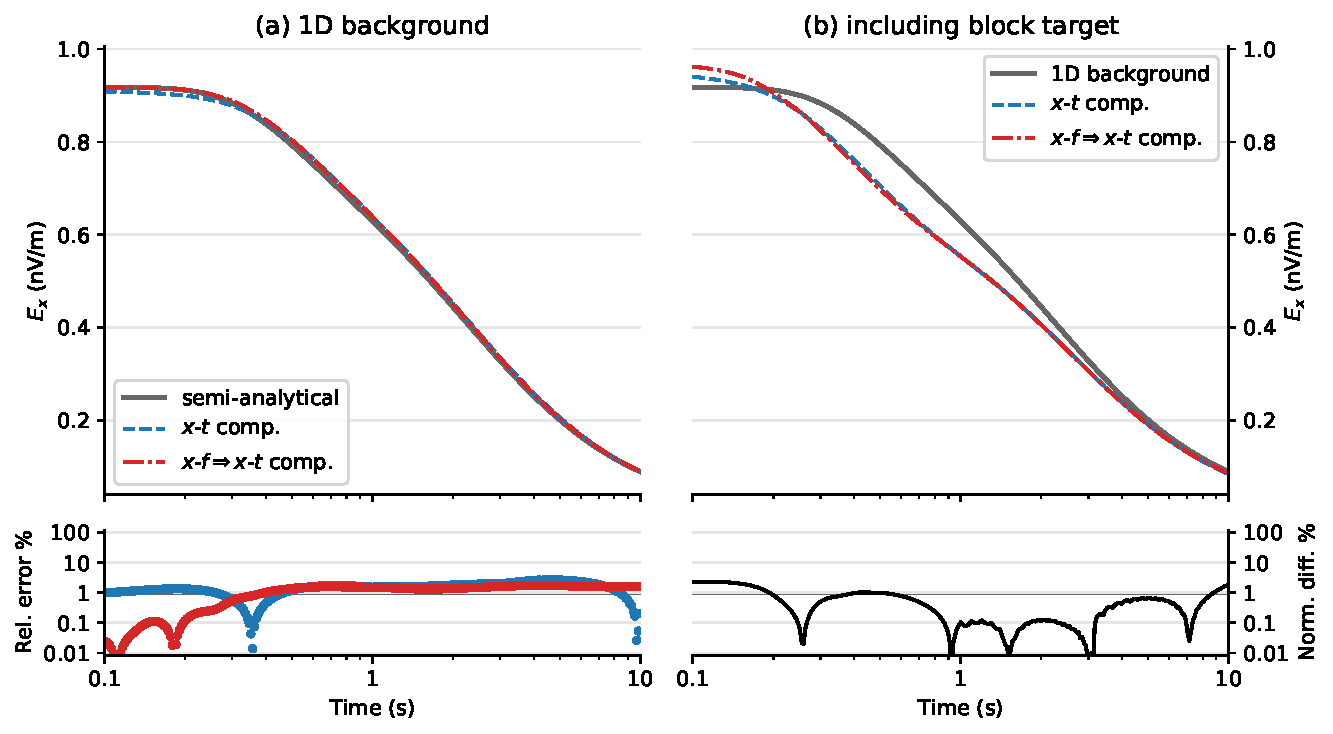
\includegraphics[width=\fwidth]{10-3d-result}
  \caption{Responses for the model outlined in Figure~\ref{fig:3d-model} using
    time-domain and frequency-domain computations, and for the layered
    background also the semi-analytical result. In the lower plot of (a) the
    relative error (\%) is shown in comparison to the semi-analytical result,
    and in (b) the normalized difference (\%) between the two 3D codes.
    \deleted{The results of these plots are clipped for values smaller than
    0.1\,\% and bigger than 10\,\%.}}
  \label{fig:3d-result}
\end{figure*}
%
The background comparison shows that both 3D codes do an acceptable job with a
relative error of a few percents at most; the result obtained through
transformation seems to be better at early times. The reason is probably the
implemented backward Euler scheme in the time-domain code that has an error of
order one in time. We cannot compare the errors for the response that includes
the target for lack of an analytical solution. The 1D background model is only
included to show that there is a significant response from the target. We
therefore show the normalized difference (NRMSD) between the two responses
$R_1$ and $R_2$ as a percentage, where $\mr{NRMSD~(\%)} = 200|R_1 - R_2|/(|R_1|
+ |R_2|)$. The NRMSD between the two codes is below 1\,\% everywhere except for
early times. Both codes took roughly 4--5 minutes to compute the two models
(single thread). However, in this particular comparison, the main difference in
runtime is not frequency-domain computation vs. time-domain computation, but
iterative solver vs. direct solver.


\subsection{\added{Induced Polarization}} % % % % % % % % % % % % % % % % % % %

\added{Note to reviewers: This entire section is new, without being all
marked in green.}

\added{mention independence of spatial complexity, why we also show 1D
examples.}

The Cole-Cole model \citep[CCM, ][]{JCP.41.Cole}, written in terms of
conductivities instead of electric permittivities as by the original authors,
is given by
%
\begin{equation}
  \sigma(\omega) = \sigma_\infty + \frac{\sigma_0 - \sigma_\infty}{1 +
    (\rm{i}\omega\tau)^c}\ ,
  \label{eq:ccm}
\end{equation}
%
where $\sigma_0$ and $\sigma_\infty$ refer to the low-frequency and
high-frequency conductivity values, respectively, $\tau$ is the central
relaxation time, and $c$ the CCM exponent describing the broadness of the
relaxation time distribution. Note that this model slightly differs from the
one phrased in terms of resistivities given by \cite{GEO.78.Pelton}, see, e.g.,
\cite{GJI.13.Tarasov}.
%
\begin{figure}
  \centering
  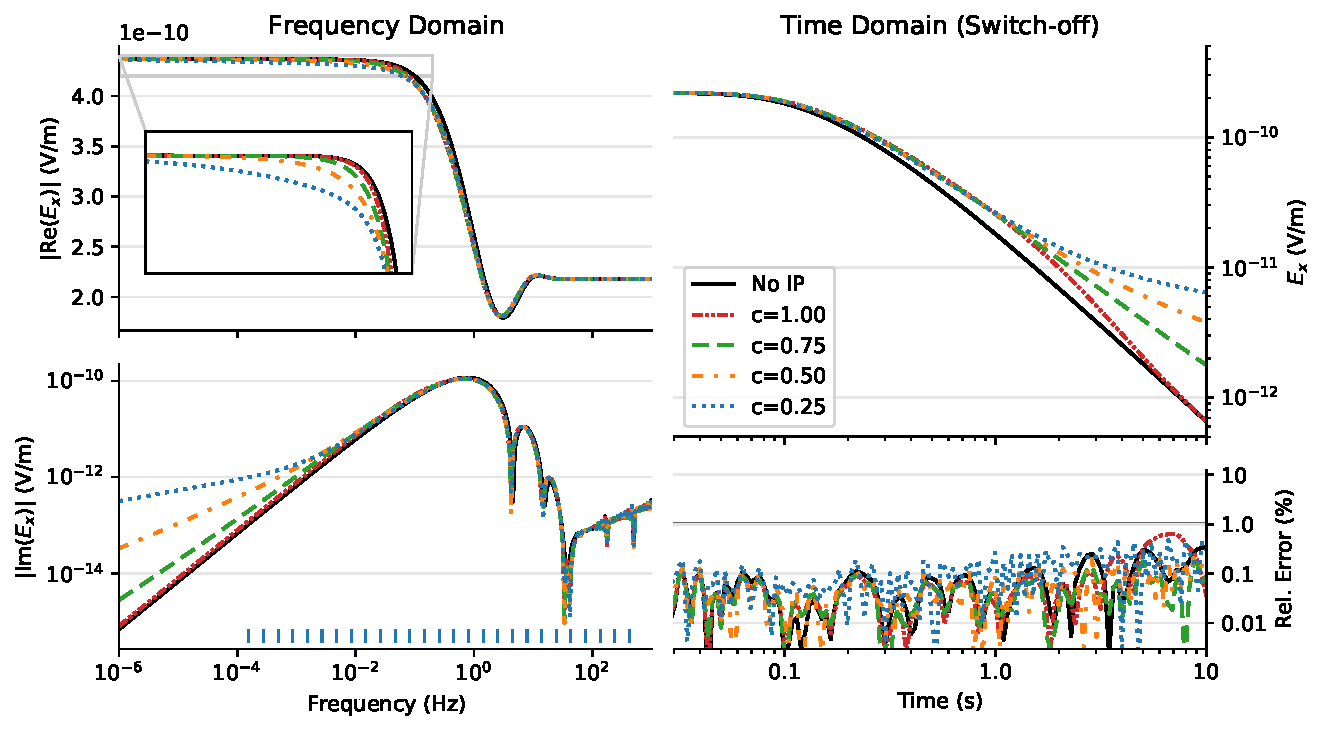
\includegraphics[width=\fwidth]{11-cole-cole-model}
  \caption{}
  \label{fig:CCM}
\end{figure}
%

It required only 30 frequencies from 1.5e-8 to 8.3\,Hz, instead of the 244
frequencies from 1.5e-8 to 6.8e6\,Hz required by the digital filter (201\,pt
filter from Key, 2012). Besides the fact that the responses for the higher
frequencies can be set to zero it is also sufficient to only compute every
5th of the required frequencies.

low frequencies cannot be 'interpolated'; however, other tricks could be
implemented. The DC values (so low frequencies or late times) is the same
independent of the IP effect. This makes it possible to estimate the DC value
with the IP-free model which does not require very low frequencies, and use
consequently this DC value to interpolate the low frequencies.


\section{Conclusions} % % % % % % % % % % % % % % % % % % % % % % % % % % % % %

We have shown a method to minimize the required frequencies and their range for
the computation of time-domain CSEM data with a frequency-domain code. This can
significantly reduce the computation time and makes time-domain CSEM modelling
with a frequency-domain code competitive given a robust frequency-domain
solver, a frequency-dependent gridding function that minimizes the required
cells, and a Fourier transform that works on a logarithmic scale. Fast layered
modelling can be used to design the required frequency range, as the Fourier
transform does not know about the dimensionality of the underlying model.
Twenty frequencies or less are usually sufficient for a wide range of offsets.
The values for lower frequencies can be interpolated using PCHIP knowing that
the imaginary part goes to zero for zero frequency. The values for higher
frequencies can be set to zero, as we can neglect their influence. And values
for frequencies in-between the computed ones are best obtained with a spline
interpolation. The actual transform can be carried out with either the DLF
method or FFTLog, where the latter one requires usually much fewer frequencies
to be interpolated. We have demonstrated the idea of our Fourier transform
method on CSEM data transformed from the frequency domain to the time domain.
However, it could equally be applied to the transform from the time domain to
the frequency domain and to other methods with similar characteristics. We
believe that our proposed improvements to the previously published methods
makes simulating results in one domain obtained through computations in the
other domain followed by a transformation a viable alternative. The methodology
is relatively simple to implement in any code.

\section{Data Availability Statement} % % % % % % % % % % % % % % % % % % % % %

The data that support the findings of this study are openly available at Zenodo
at \href{https://zenodo.org/badge/DOI/10.5281/zenodo.???????}{doi:
10.5281/zenodo.???????}. The data includes the scripts and instructions to
reproduce all results and figures.

\emph{Note to editors and reviewers: The data are NOT YET on Zenodo, we will
upload there the final versions and link the right DOI for the final
manuscript. Until then everything can be found on GitHub at
\href{https://github.com/empymod/article-TDEM}%
{github.com/empymod/article-TDEM}.}


\begin{acknowledgments} % % % % % % % % % % % % % % % % % % % % % % % % % % % %
This research was conducted within the Gitaro.JIM project funded through
MarTERA as part of Horizon 2020, a funding scheme of the European Research Area
(ERA-NET Cofund, \href{https://www.martera.eu}{martera.eu}). An early idea of
this manuscript was presented by \cite{EAGE.20.Werthmuller}.
\end{acknowledgments}


% REFERENCES
\bibliographystyle{gji}
\bibliography{Refs}

\label{lastpage}

\end{document}
